\usepackage{lipsum}
\usepackage[a4paper,top=2cm,bottom=2cm,inner=3cm,outer=1cm,marginparwidth=4cm]{geometry}
\usepackage{titlesec}
\usepackage{titling}
\usepackage{fontspec}
\usepackage{suffix}
\usepackage{multicol}
\usepackage{tikz}
\usepackage{pdflscape}
\usepackage{onimage} % loaded to print tikz on images
\usepackage{bm}
\usepackage{textcomp}
\usepackage{gensymb}
\usepackage{enumitem}

% ---- watermark
\usepackage{eso-pic}
\newcommand\FrontPic{%
\put(0,0){%
\parbox[b][\paperheight]{\paperwidth}{%
\vspace*{.3\paperheight}
\flushleft
\includegraphics[height=.7\paperheight,%
keepaspectratio]{img/front.png}%
\vfill
}}}

\newcommand\BackPic{%
\put(0,0){%
\parbox[b][\paperheight]{\paperwidth}{%
\vspace*{.3\paperheight}
\flushright
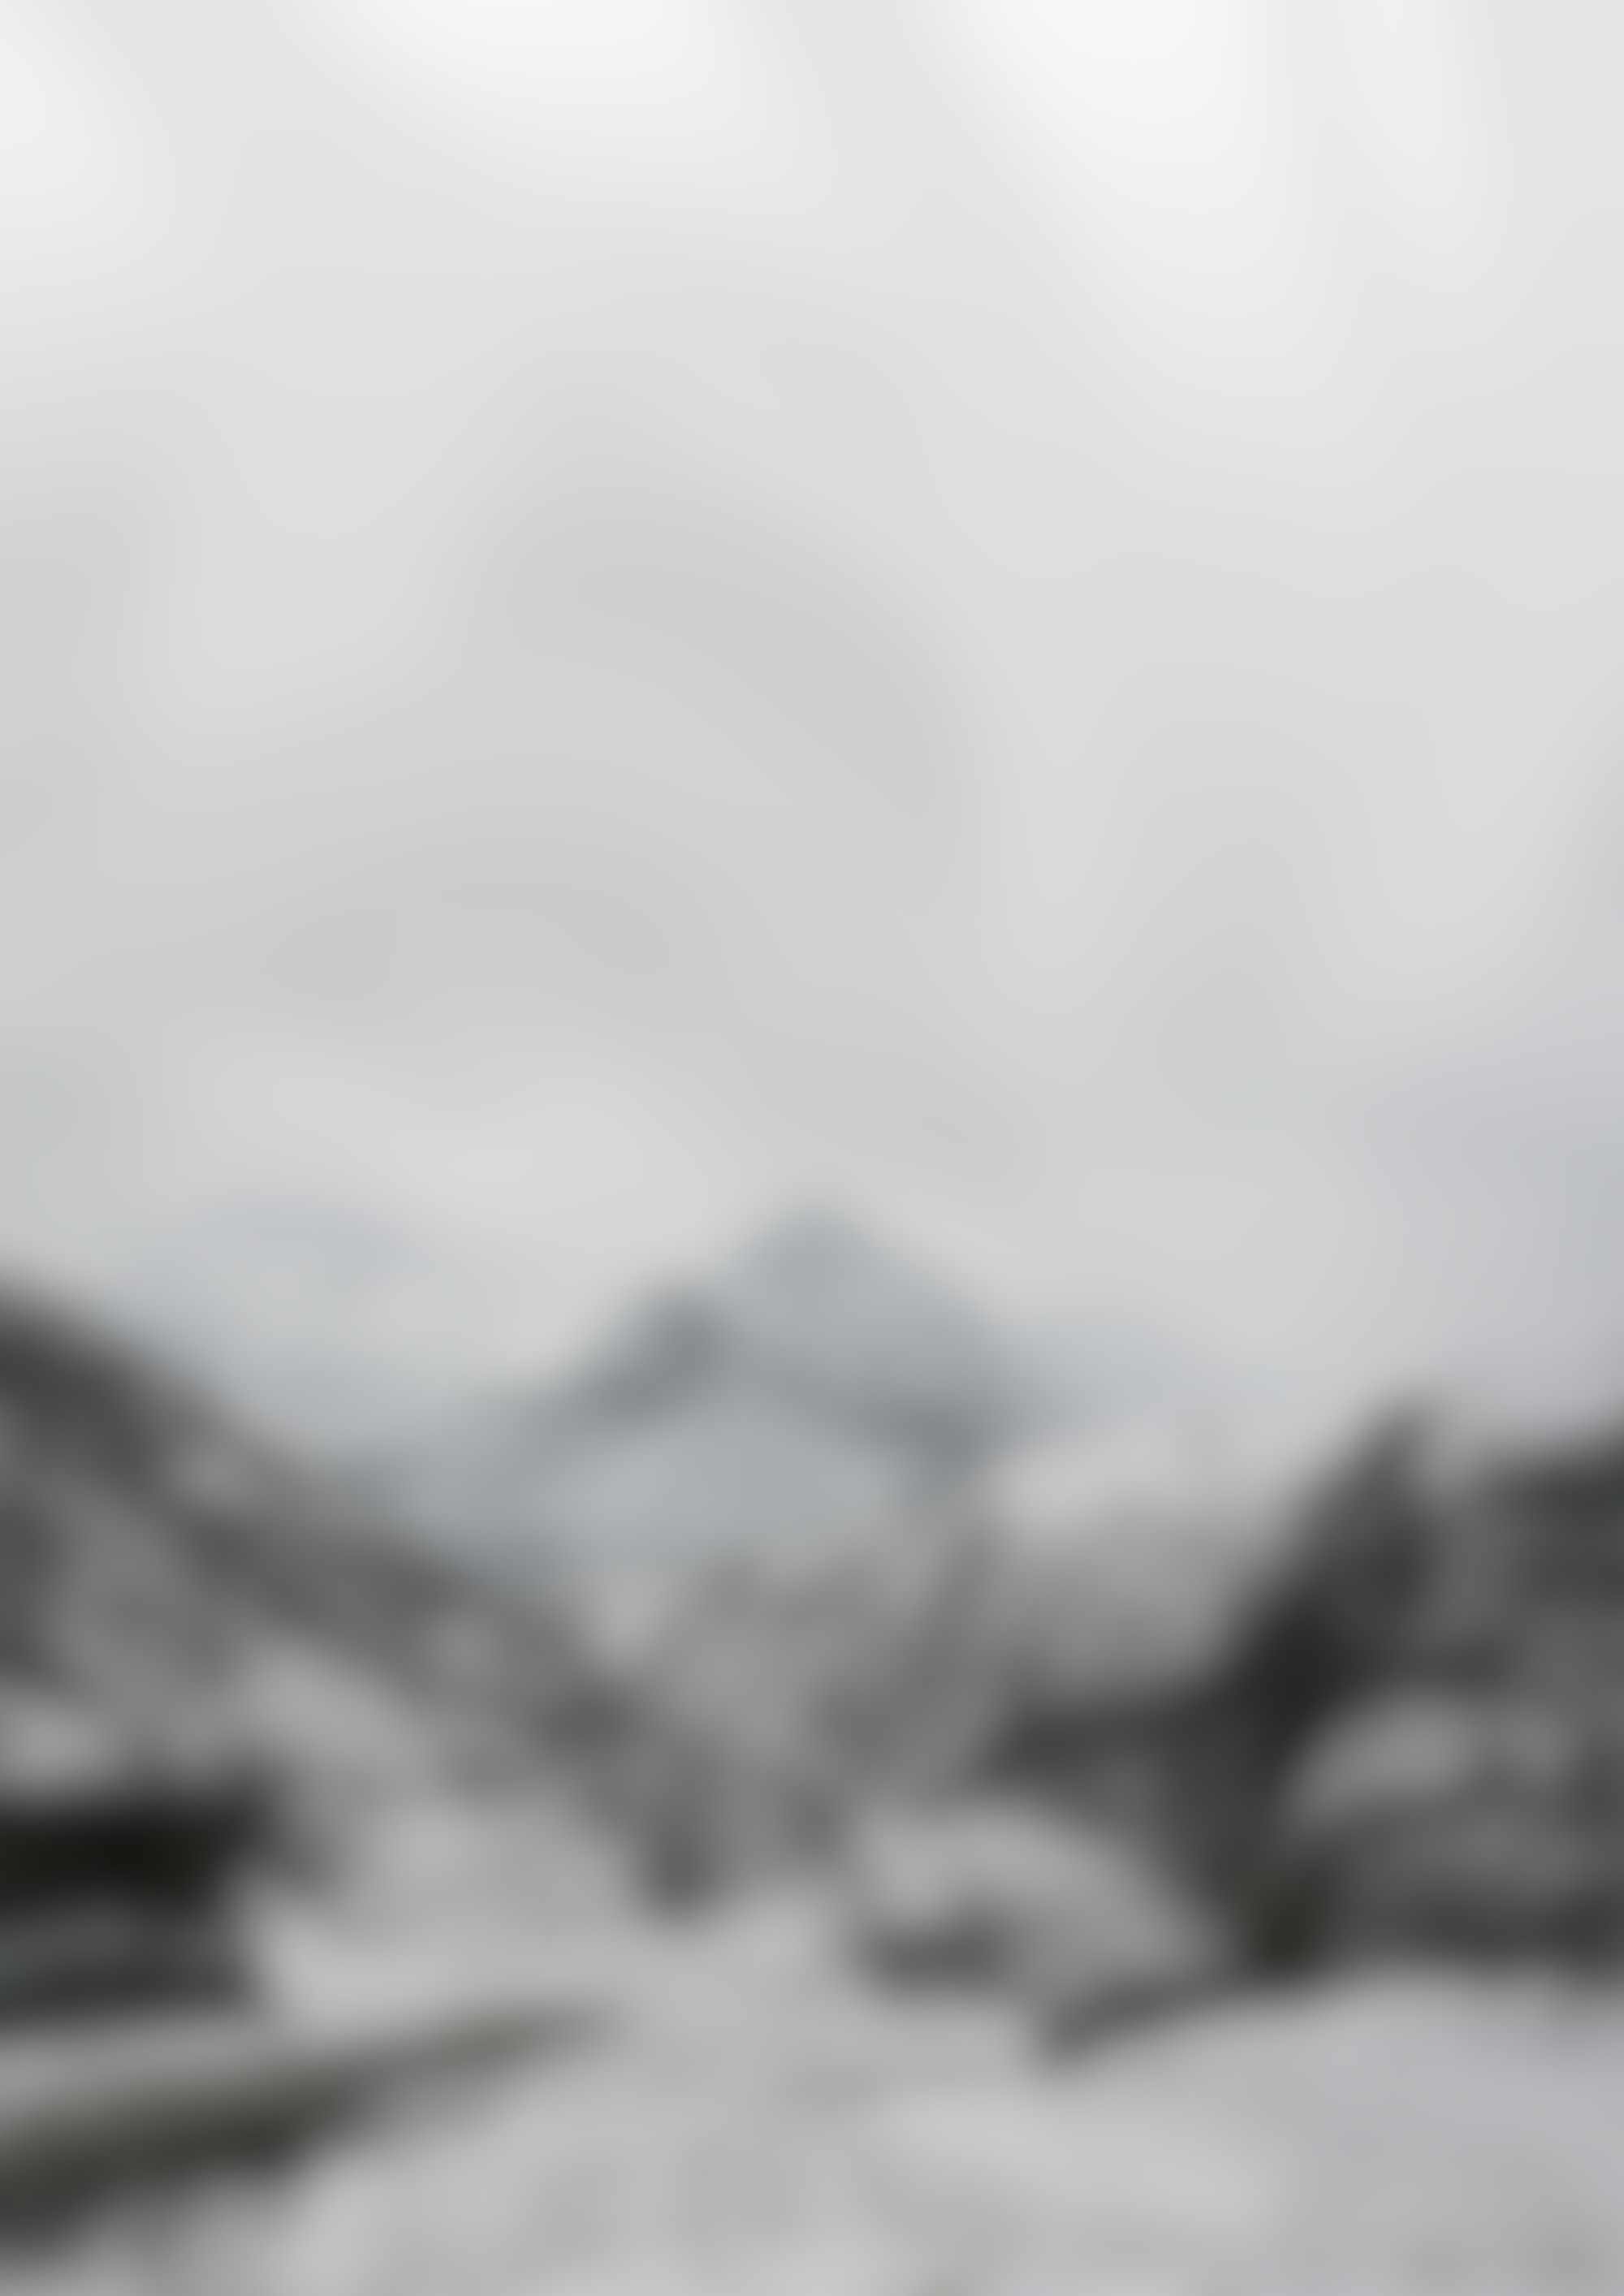
\includegraphics[height=.7\paperheight,%
keepaspectratio]{img/back.png}%
\vfill
}}}

\newcommand{\NewPic}[1]{
\put(0,0){%
\parbox[b][\paperheight]{\paperwidth}{%
\vspace*{.22\paperheight}
\flushright
\includegraphics[width=1\paperwidth,%
keepaspectratio]{#1}%
\vfill
}}}

\newcommand{\NewPicHeight}[2]{
\put(0,0){%
\parbox[b][\paperheight]{\paperwidth}{%
\vspace*{#2}
\flushright
\includegraphics[width=1\paperwidth,%
keepaspectratio]{#1}%
\vfill
}}}

\usepackage{xcolor}%,sectsty}
\definecolor{clrt1}{RGB}{215, 95, 95}    % color 1
\definecolor{clrt2}{RGB}{135, 175, 135}  % color 2
%\definecolor{clrt1}{RGB}{80, 80, 80}    % gray 1
%\definecolor{clrt2}{RGB}{180, 180, 180}  % gray 2

%\newcommand{\code1}[1]{\textcolor{clrt1}{#1}}

\usepackage{tocloft}
\renewcommand{\cftchapfont}{\color{clrt1}}
\renewcommand{\cftsecfont}{\color{clrt2}}

\newcommand\chapterauthor[5]{\authortoc{#1}{#4}{#5}\noindent\printchapterauthor{#1}{#2}{#3}}
\WithSuffix\newcommand\chapterauthor*[1]{\printchapterauthor{#1}{}{}}

\makeatletter
\newcommand{\printchapterauthor}[3]{%
  {%\vspace*{-25pt}%
  %\linespread{1.5}
  \large#1$^{~\small\textnormal#2}$#3%
  %\par\nobreak\vspace*{30pt}
  }
  \@afterheading%
}

\newcommand{\authortoc}[3]{%
  \addtocontents{toc}{\hspace{#2em}}%\vskip-10pt}%
  \addtocontents{toc}{
    {\protect\scriptsize\textcolor{black}{#1#3}}{}{}
    }
  %\addtocontents{toc}{\vskip5pt}%
}

\setmainfont{Charter}[
  Path=./fnt-charter/,
  Extension=.ttf,
  UprightFont=*-Regular,
  BoldFont=*-Bold,
  ItalicFont=*-Italic,
  BoldItalicFont=*-Bold-Italic
]

\usepackage{titling}

% paragraph formating -----------
\setlength\fboxsep{.6em}
\setlength{\parskip}{.8em} % vertical spcae
\setlength{\parindent}{0em} % vertical spcae
\renewcommand{\baselinestretch}{1.2} 

\newcommand{\headchapter}{}

\usepackage{fancyhdr}
 \setlength{\headheight}{15pt} 
\pagestyle{fancy}
\fancyhf{}
%\rhead{\chaptername \headchapter}
\fancyhead[RO, LE] {\chaptername \headchapter}
\cfoot{--~\thepage~--}

\newcommand\mystyleone{%
\fancyhf{}
%\rhead{\chaptername \headchapter}
\fancyhead[RO, LE] {\chaptername \headchapter}
\cfoot{--~\thepage~--}
}
 
\newcommand\mystyletwo{%
   \cfoot{--~\thepage~--}
}


%title formatin (margins)
\titlespacing\chapter{0pt}{0em plus 4pt minus 2pt}{1em plus 2pt minus 2pt}
\titleformat{\chapter}{\Huge\normalfont\bfseries\color{clrt1}}{}{0em}{\hfil{--\hspace*{.25em}\thechapter\hspace*{.25em}-- }\\}
\titleformat{\section}{\large\bfseries\color{clrt2}}{\thesection.}{0.5em}{}
% table formats  -----------
\usepackage{multirow}
\usepackage{multicol}
\usepackage{colortbl}
\usepackage{array}
\newcolumntype{L}[1]{>{\raggedright\let\newline\\\arraybackslash\hspace{0pt}}m{#1}}
\newcolumntype{C}[1]{>{\centering\let\newline\\\arraybackslash\hspace{0pt}}m{#1}}
\newcolumntype{R}[1]{>{\raggedleft\let\newline\\\arraybackslash\hspace{0pt}}m{#1}}

% citation management -----------
\newcommand{\cc}[1]{\textcolor{clrt2!80}{#1}}
\newcommand{\dd}[1]{\textcolor{clrt1!80}{#1}}
\newcommand{\gitref}{\hyperlink{git}{git}}
\newcommand{\textsw}[1]{\textcolor{darkgray}{\textsc{#1}}}
% defining the comand \mean to draw a bar over a math expression to indicate the mean
\newcommand{\overbar}[1]{\mkern 1.5mu\overline{\mkern-1.5mu#1\mkern-1.5mu}\mkern 1.5mu}
\newcommand*\mean[1]{\overbar{#1}}

% setting up link colors
\usepackage{hyperref}
\hypersetup{
    colorlinks,
    linkcolor={black!60},
    citecolor={black!60},
    urlcolor={black!60}}

% bibliography management -----------
% inline citations
\usepackage{csquotes}
\makeatletter
%Take the original environment definition and change the left margin
\renewenvironment*{displayquote}
  {\begingroup\setlength{\leftmargini}{1.3em}\csq@getcargs{\csq@bdquote{}{}}}
  {\csq@edquote\endgroup}
\makeatother

\usepackage{bibentry}
\usepackage{natbib}  %set citing format
\bibliographystyle{apalike}
%\makeatletter 
%\renewcommand\@biblabel[1]{#1.} 
%\makeatother
\usepackage{multibib}
\newcites{at}{\normalsize\textcolor{black}{Original publication}}
\newcites{am}{Chapter 1 References}

\newcites{bt}{\normalsize\textcolor{black}{Original publication}}
\newcites{bm}{Chapter 2 References}

\newcites{ct}{\normalsize\textcolor{black}{Original publication}}
\newcites{cm}{Chapter 3 References}

\newcites{dt}{\normalsize\textcolor{black}{Original publication}}
\newcites{dm}{Chapter 4 References}

\newcites{im}{Intro References}
\newcites{zm}{Synthesis References}

\usepackage{etoolbox}
\makeatletter
\providecommand{\bibname}{Bibliography}
\providecommand{\refname}{References}
\@ifpackageloaded{natbib}
  {\renewcommand{\bibsection}{%
    \@ifundefined{chapter}
    {\subsection*{\refname \markboth{\refname}{\bibname}%
    \addcontentsline{toc}{subsection}{\refname}}
    }
    {\section*{\refname \markboth{\refname}{\bibname}%
    \addcontentsline{toc}{section}{\refname}}
    }
  }}
  {\@ifundefined{chapter}
    {\patchcmd{\thebibliography}{\section*{\refname}}{%
      \subsection*{\refname}
      \addcontentsline{toc}{subsection}{\refname}
      }{}{}
    }
    {\patchcmd{\thebibliography}{\chapter*{\bibname}}{%
      \section*{\refname}
      \addcontentsline{toc}{section}{\refname}
      }{}{}
    }
  }
\@ifundefined{chapter}
  {\newcommand{\bibliographies}{%
  \section*{\bibname}
  \if@FMB@addtotoc\addcontentsline{toc}{section}{\bibname}\fi}}
  {\newcommand{\bibliographies}{%
  \chapter*{\bibname}
  \if@FMB@addtotoc\addcontentsline{toc}{chapter}{\bibname}\fi}}
\makeatother

% figure/table management -----------
\usepackage{floatrow}
\usepackage[figurename=Figure,tablename=Table,labelfont=bf,format=plain, font=footnotesize]{caption} 
\captionsetup[figure]{labelfont={bf},labelformat={default},labelsep=colon}
\floatsetup[table]{capposition=top}

\newcounter{figS}
\newcommand{\figS}[1]{\refstepcounter{figS}\label{#1}}
\newcounter{tabS}
\newcommand{\tabS}[1]{\refstepcounter{tabS}\label{#1}}

\newcommand{\figref}[1]{\hyperref[#1]{Figure~\ref{#1}}}
\newcommand{\tabref}[1]{\hyperref[#1]{Table~\ref{#1}}}
\newcommand{\figrefS}[1]{\hyperref[#1]{Suppl. Fig.~\ref{#1}}}
\newcommand{\tabrefS}[1]{\hyperref[#1]{Suppl. Tab.~\ref{#1}}}

\usepackage{placeins}
\DeclareFloatingEnvironment[
  fileext=losf,
  listname={List of Supplementary Figures},
  name=Suppl.~Figure
]{supplFigure}

\DeclareFloatingEnvironment[
  fileext=lost,
  listname={List of Supplementary Tables},
  name=Suppl.~Table
]{supplTable}


\newlength{\fwidth}
\setlength{\fwidth}{168.36mm}%{183mm}
\newlength{\fheight}
\setlength{\fheight}{261.28mm}%{284mm}

\titlespacing*{\chapter}{0pt}{-50pt}{40pt}

\usepackage{morewrites}
%take out later
\usepackage{colortbl}
\definecolor{annoGRAY}{RGB}{240,240,240}
\definecolor{annoDGRAY}{RGB}{200,200,200}
\newcommand{\gene}[1]{\textit{\MakeLowercase{#1}}}

%\renewcommand{\cftloftitlefont} {\MakeUppercase{\large\bfseries}}
%\renewcommand{\cftlottitlefont} {\MakeUppercase{\large\bfseries}}
\renewcommand{\listfigurename}{\textcolor{clrt2}{\large\textbf{List of Figures}}}
\renewcommand{\listsupplFigurename}{\textcolor{clrt2}{\large\textbf{List of Supplementary Figures}}}

\renewcommand{\listtablename}{\textcolor{clrt2}{\large\textbf{List of Tables}}}
\renewcommand{\listsupplTablename}{\textcolor{clrt2}{\large\textbf{List of Supplementary Tables}}}

% keep last line of paragraph justified
\newcommand{\startsquarepar}{%
    \par\begingroup \parfillskip 0pt \relax}
\newcommand{\stopsquarepar}{%
    \par\endgroup}
    
\usepackage[most]{tcolorbox}

\newcommand{\projanticase}[1]{\MakeUppercase{#1}}
\newcommand{\projcase}[1]{\MakeLowercase{#1}}
\usepackage{amssymb}

\newcommand\blankpage{%
    \clearpage\thispagestyle{empty}\mbox{}\clearpage
%    \addtocounter{page}{-1}%
    \newpage}
    
% manual code highlighting
\usepackage{listings}
\lstset{
  basicstyle=\ttfamily,
  escapeinside=||
}

\newcommand{\coderule}{\textcolor{black!35}{\hfil\rule{.98\linewidth}{0.2pt}}}
